%!TEX TS-program = xelatex
\documentclass[]{friggeri-cv}
\usepackage{afterpage}
\usepackage{hyperref}
\usepackage{color}
\usepackage{xcolor}
\usepackage{fancyhdr}
\pagestyle{fancy}
\lhead{}
\chead{}
\rhead{}
\rfoot{{\footnotesize {See the last version of this document at: \href{https://github.com/diraol/cv/blob/tex-pdf-version/cv.pdf}{https://github.com/diraol/cv/blob/tex-pdf-version/cv.pdf}}}}
\renewcommand{\headrulewidth}{0pt}
\renewcommand{\footrulewidth}{0pt}

\hypersetup{
    pdftitle={Diego Rabatone Oliveira Resume},
    pdfauthor={Diego Rabatone Oliveira},
    pdfsubject={Resume/CV},
    pdfkeywords={Diego Rabatone, diraol, cv, resume},
    colorlinks=false,       % no lik border color
   allbordercolors=white    % white border color for all
}
\addbibresource{bibliography.bib}
\RequirePackage{xcolor}
\definecolor{pblue}{HTML}{0395DE}

\begin{document}
\thispagestyle{empty}
\pagenumbering{gobble}% Remove page numbers (and reset to 1)
\header{Diego}{Rabatone O.}
      {Computer Engineer}
      
% Fake text to add separator      
\fcolorbox{white}{gray}{\parbox{\dimexpr\textwidth-2\fboxsep-2\fboxrule}{%
.....
}}

% In the aside, each new line forces a line break
\begin{aside}
  \section{Address}
    São Paulo, SP, Brazil
    ~
  \section{Tel}
    +55 11 9-8231-4249
    ~
  \section{Mail}
    \href{mailto:diraol@diraol.eng.br}{\textbf{diraol@}\\diraol.eng.br}
    \href{mailto:diraol@usp.br}{\textbf{diraol@}\\usp.br}
    ~
  \section{IRC}
    \#diraol (at) irc.freenode.net
    ~
  \section{Twitter}
    \href{http://twitter.com/diraol}{@diraol}
    ~
  \section{Web \& Git}
    \href{http://cv.diraol.eng.br}{cv.diraol.eng.br}
    \href{https://github.com/diraol}{github.com/diraol}
    ~
  \section{Programming}
    Python
    JavaScript
    CSS
    ShellScript
    R
    \LaTeX
    \href{http://ghv.artzub.com/\#user=diraol}{ghv.artzub.com/}
    \href{http://ghv.artzub.com/\#user=diraol}{\#user=diraol}
    ~
  \section{Daily OS}
    Debian GNU/Linux\\%
\includegraphics[scale=0.40]{img/5stars.png}
    Gnome3\\%
\includegraphics[scale=0.40]{img/2stars.png}
    Vim
    ~
  \section{Other Techs}
    Nginx
    Varnish
    Xen
    MySQL
    Postgres
    CartoDB
    QuantumGis
    Inkscape
    Gimp
\end{aside}

\section{Experience}
\begin{entrylist}
  \entry
    {07/12 - Now}
    {Digital Media Analist}
    {O Estado de S.Paulo S/A}
    {Main developer of the data driven journalism team ("\href{http://estadaodados.com}{Estadão Dados}").\\
     Responsabilities:\\
     DataViz - From concept creation to full deploy, usually web interactive\\
     Data Analysis - Analysis of public databases of any area of knowledge\\
     Data Scraping - Gathering public data mostly with python crawlers\\
     Data Treatment - Cleaning and structuring databases to be analysed\\
     \href{http://estadaodados.com}{http://estadaodados.com}\\}
  \entry
    {10/09 - now}
    {Co-Founder, coordinator and member}
    {\href{http://polignu.org}{PoliGNU}}
    {PoliGNU - Poli-USP Free Software Studies Group\\
    Organization and planning of activities and discussion groups\\
     Infrastructure management (SysAdmin, website)\\
     Disclosure and presentation at conferences, seminars, workshops, etc\\
     \href{http://polignu.org}{http://polignu.org}}
   \entry
    {07/08 - 12/13}
    {Volunteer SysAdmin}
    {Escritório Piloto - Poli-USP}
    {Design and Setup of LAN, with OpenLDAP server, File Sharing (NFS), WebServer, Virtualization (XEN) and local DNS Server\\
     Design, development and management of an institucional website on Drupal\\}
   \entry
    {08/10 - 08/11}
    {Math Teacher}
    {ACEPUSP}
    {Math teacher on a preparatory course to low income students\\}
   \entry
    {08/10 - 12/10}
    {Volunteer}
    {Universidade de São Paulo}
    {Database modeling for the new version of the Teaching Evaluation System\\}
   \entry
    {01/09 - 08/10}
    {Volunteer}
    {Escola de Governo}
    {Design, development and management of institucional website on Joomla\\
     Orientation and Mentoring of Governor Formation Course Students\\}
   \entry
    {03/05 - 06/06}
    {Fellow}
    {Universidade de São Paulo}
    {Developer of the first Digital Teaching Evaluation System}
\end{entrylist}

\section{Education}
\begin{entrylist}
  \entry
    {2005 - 2014}
    {Undergraduate in Computer and Digital Systems Engineering\\}
    {Universidade de São Paulo, Brazil}
    {Conclusion in 2014\\
    %Main subjects: Matematics and Physics, Programming, Operational Research, Telecommunication Systems, Digital and Analogical Electronics.\\
    %\emph{Title of the Thesis: "Development, Management and Migrations of web contents and applications".}\\
    %\emph{Thesis activity carried out during an internship period at Atitlan Engineering SRL.}\\
    }
  \entry
    {2000 - 2002}
    {High School}
    {Colégio Rio Branco, São Paulo, Brasil}
    {%Scientific Secondary School.\\
    %Main subjects: Matematics, Physics, Computer Science.
    }
\end{entrylist}

%\section{Certifications}
%\begin{entrylist}
%  \entry
%    {02/2013}
%    {Intro to Computer Science}
%    {Udacity. E-learning}
%    {\emph{Building a Python Search Engine}}
%\end{entrylist}

\newpage
\pagenumbering{gobble}% Remove page numbers (and reset to 1)
\begin{aside}
~
~
~
%  \section{Places Lived}
%    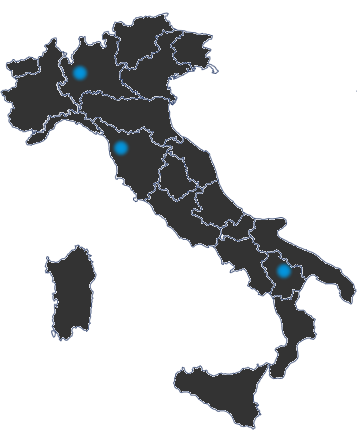
\includegraphics[scale=0.25]{img/italia.png}
%    ~
  \section{Languages}
    \textbf{Portuguese}
\includegraphics[scale=0.40]{img/5stars.png}
    \textbf{English}
\includegraphics[scale=0.40]{img/5stars.png}
    \textbf{French}
\includegraphics[scale=0.40]{img/1stars.png}
    \textbf{Spanish}
\includegraphics[scale=0.40]{img/1stars.png}
~    
  \section{Jung Typology Test - INFJ}
    \textbf{I}ntrovert {\footnotesize (11\%)}
    I\textbf{n}tuitive {\footnotesize (50\%)}
    \textbf{F}eeling   {\footnotesize (12\%)}
    \textbf{J}udging   {\footnotesize (44\%)}
    \href{http://www.humanmetrics.com/hr/JTypesResult.aspx?EI=-11&SN=-50&TF=-12&JP=44}{\footnotesize Click for result}
    \href{http://www.humanmetrics.com/personality/infj}{\footnotesize INFJ Desc}
~
  \section{Personal Skills}
    Empathy
    
\includegraphics[scale=0.40]{img/5stars.png}
    Integrity
    
\includegraphics[scale=0.40]{img/5stars.png}
    Social Boldness
    
\includegraphics[scale=0.40]{img/5stars.png}
    Team Working
    
\includegraphics[scale=0.40]{img/4stars.png}
    Emotional Intelligence
    
\includegraphics[scale=0.40]{img/4stars.png}
    {\footnotesize test from \href{http://www.skillsyouneed.com/ips/interpersonal-skills-test.html}{SkillsYouNeed.com}}
    {\footnotesize Interpersonal Skills Test}
    %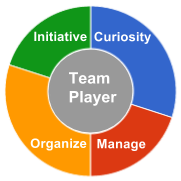
\includegraphics[scale=0.62]{img/personal.png}
    ~
  \section{Hobbies}
      \href{http://olhares.com/diraol}{Photograpy}
      Tae-Kwon-Do
\end{aside}

\section{Publications}
\textbf{Twitter API, ElasticSearch e Kibana - Analisando a rede social}\\
\emph{Tutorial on how to gather, process and analyse twitter traffic}\\
\href{http://polignu.org/artigo/twitter-api-elasticsearch-e-kibana-analisando-rede-social}{http://polignu.org/artigo/twitter-api-elasticsearch-e-kibana-analisando-rede-social}

\textbf{DiRaOLinux}\\
\emph{Blog to document and share daily discovers and issues fixes}\\
\href{http://diraol.polignu.org}{http://diraol.polignu.org}

\textbf{Caderno do PoliGNU - Vol 1 - Software e Cultura Livres}\\
\emph{Introductory material about Free Software and Free Culture (pt-br)}\\
\href{http://polignu.org/administrativo/caderno-polignu-volume-1-software-e-culturas-livres}{http://polignu.org/administrativo/caderno-polignu-volume-1-software-e-culturas-livres}

\section{Projects}
\textbf{The Parliamentary Radar} - \href{http://radarparlamentar.polignu.org/}{http://radarparlamentar.polignu.org/}\\
It's a web application that determinates "similarities" between political parties based on the analysis of voting data of legislative houses. There are also some gender analysis from the Parliament. 
This project has been received 4 awards since 2012.\\
Technologies: Django/Python, R, SQLite/MySQL/Postgres, nginx, uWSGI, D3.js

\textbf{Transparência Hacker (\textit{Hacker Transparency})}\\
Member of Brazilian Hacker Transparency community, that advocates for OpenGov, Public Transparency, OpenData, etc. The community created the HackerBus, participated on the creation of a HackerLab at the Congress, influenced the Brazilian Public Information Access act and the ``Marco Civil da Internet'', besides other projects.\\
HackLab at Congress: \href{http://blog.openingparliament.org/post/72099651071/a-permanent-hacker-space-in-the-brazilian-congress}{http://blog.openingparliament.org/post/72099651071/a-permanent-hacker-space-in-the-brazilian-congress}
\section{Events}
07/14 - \href{http://abraji.org.br/congresso/}{\textbf{9$^{th}$ Internation Investigative Journalism Congress}}\\
Instructor of the "Coding for journalists" workshop.

11/13 - \href{https://knightcenter.utexas.edu/pt-br/blog/00-14390-inscricoes-abertas-para-primeiro-curso-da-anj-com-o-centro-knight-introducao-ao-jornal}{\textbf{Introduction to Data Journalism MOOC}}\\
Instructor of the "Programming" module of the cours. This course was organized by Knight Center and the brazilian National Journals Association

11/13 - \href{http://2.encontro.dados.gov.br/encontro.html}{\textbf{II Brazilian National Conference of OpenData}}\\
Chairman of the dataviz trail

07/13 - \href{http://rodadahacker.com/}{\textbf{II RodAda Hacker}}\\
Mentor on the second edition of "Rodada Hacker", a one day workshop that aims to give woman autonomy with techonologies

05/13 - \href{http://www2013.org/}{\textbf{www2013 Conference}}\\
Speaker on the "eGov and Open Data Camp" discussion, talking about "The challenges and opportunities of data journalism"

03/13 - \href{http://rodadahacker.com/}{\textbf{I RodAda Hacker}}\\
Mentor on the first edition of "Rodada Hacker", a one day workshop that aims to give woman autonomy with techonologies

10/12 - \href{http://yapcbrasil.org.br/2012/talk/110}{\textbf{YAPC::Brasil 2012}}\\
"The Parliamentary Radar: Unraveling the legislative politics"

05/10 - \href{http://artigo19.org/infoedireitoseu/?p=560}{\textbf{The Right to Information Access}}\\
Speaker about the Right to Information Access at PUC Univeristy
%
%\\
%
%\begin{flushleft}
%\emph{November 22th, 2014}
%\end{flushleft}
%\begin{flushright}
%
%\end{flushright}
%
%%% This piece of code has been commented by Karol Kozioł due to biblatex errors. 
% 
%\printbibsection{article}{article in peer-reviewed journal}
%\begin{refsection}
%  \nocite{*}
%  \printbibliography[sorting=chronological, type=inproceedings, title={international peer-reviewed conferences/proceedings}, notkeyword={france}, heading=subbibliography]
%\end{refsection}
%\begin{refsection}
%  \nocite{*}
%  \printbibliography[sorting=chronological, type=inproceedings, title={local peer-reviewed conferences/proceedings}, keyword={france}, heading=subbibliography]
%\end{refsection}
%\printbibsection{misc}{other publications}
%\printbibsection{report}{research reports}

\end{document}
